\section{Conclusions}\label{sec:conclusions}

For the various models the final accuracy and 0-1 loss was given.
Those metrics are good to express concisely the evaluation of a model.

We can go deeper with our insight by measuring other metrics before drawing conclusions as reported in the Figures: \ref{fig:figure2}, \ref{fig:figure3}, \ref{fig:figure4}, \ref{fig:figure5} and \ref{fig:figure6}.
% Model 1 handcrafted
% Muffin: precision=0.8419117647058824, recall=0.9308943089430894, F1=0.8841698841698841
%Chihuahua: precision=0.946875, recall=0.8757225433526011, F1=0.9099099099099098
% Model 2 handcrafted
% Muffin: precision=0.8951310861423221, recall=0.8786764705882353, F1=0.8868274582560297
% Chihuahua: precision=0.8984615384615384, recall=0.9125, F1=0.9054263565891473



\begin{figure}
    \centering
    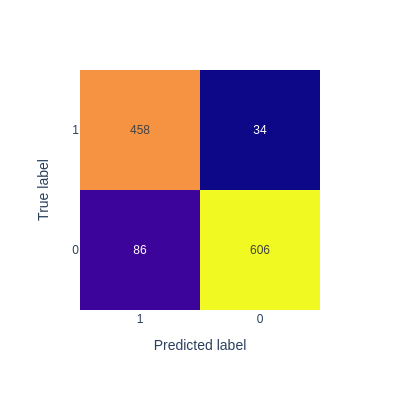
\includegraphics[scale=0.4]{/home/jacopo/PycharmProjects/muffin-stat-project/report/imgs/cnn_model_1_final_confusion}
    \begin{tabular}{ c | c | c | c| c}
        \hline
        reference  & $precision$ & $recall$ & $f1$   & $support$ \\
        \hline\hline
        muffin     & 0.8419      & 0.9309   & 0.8842 & 544       \\
        \hline
        chihuahua  & 0.9469      & 0.8757   & 0.9099 & 640       \\
        \hline
        $accuracy$ & -           & -        & 0.8986 & 1184      \\
        \hline
    \end{tabular}
    \caption{
        Metrics of the first CNN developed model
    }\label{fig:figure2}
\end{figure}


\begin{figure}
    \centering
    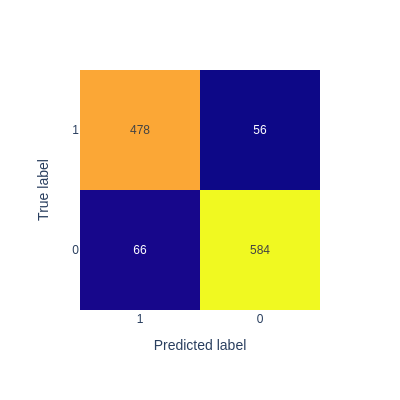
\includegraphics[scale=0.4]{/home/jacopo/PycharmProjects/muffin-stat-project/report/imgs/cnn_model_2_final_confusion}
    \begin{tabular}{ c | c | c | c| c}
        \hline
        reference  & $precision$ & $recall$ & $f1$   & $support$ \\
        \hline\hline
        muffin     & 0.8951      & 0.8787   & 0.8868 & 544       \\
        \hline
        chihuahua  & 0.8985      & 0.9125   & 0.9054 & 640       \\
        \hline
        $accuracy$ & -           & -        & 0.8970 & 1184      \\
        \hline
    \end{tabular}
    \caption{
        Metrics of the second CNN developed model
    }\label{fig:figure3}
\end{figure}


% Best CNN Autotuned model
% Muffin: precision=0.9023090586145648, recall=0.9338235294117647, F1=0.9177958446251129
% Chihuahua: precision=0.9420289855072463, recall=0.9140625, F1=0.9278350515463918

\begin{figure}
    \centering
    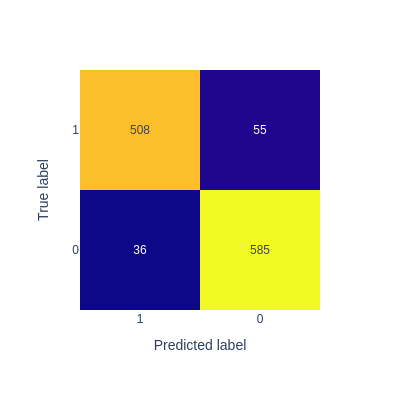
\includegraphics[scale=0.4]{/home/jacopo/PycharmProjects/muffin-stat-project/report/imgs/cnn_best_confusion}
    \begin{tabular}{ c | c | c | c| c}
        \hline
        reference  & $precision$ & $recall$ & $f1$   & $support$ \\
        \hline\hline
        muffin     & 0.9023      & 0.9338   & 0.9178 & 544       \\
        \hline
        chihuahua  & 0.9420      & 0.9141   & 0.9278 & 640       \\
        \hline
        $accuracy$ & -           & -        & 0.9231 & 1184      \\
        \hline
    \end{tabular}
    \caption{
        Metrics of the autotuned CNN model
    }\label{fig:figure4}
\end{figure}

% Xception
%Muffin: precision=0.989010989010989, recall=0.9926470588235294, F1=0.9908256880733946
%Chihuahua: precision=0.9937304075235109, recall=0.990625, F1=0.9921752738654148
\begin{figure}
    \centering
    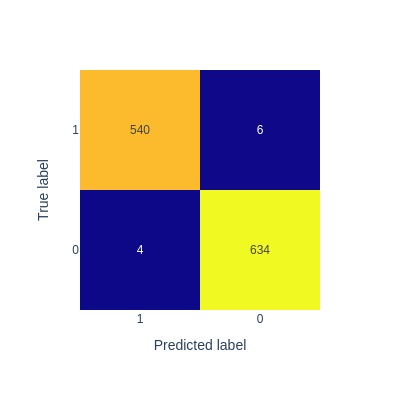
\includegraphics[scale=0.4]{/home/jacopo/PycharmProjects/muffin-stat-project/report/imgs/xception_confusion}
    \begin{tabular}{ c | c | c | c| c}
        \hline
        reference  & $precision$ & $recall$ & $f1$   & $support$ \\
        \hline\hline
        muffin     & 0.9890      & 0.9926   & 0.9908 & 544       \\
        \hline
        chihuahua  & 0.9937      & 0.9906   & 0.9922 & 640       \\
        \hline
        $accuracy$ & -           & -        & 0.9916 & 1184      \\
        \hline
    \end{tabular}
    \caption{
        Metrics of the Xception transfer learned model
    }\label{fig:figure5}
\end{figure}

% VGG16
%Muffin: precision=0.9962825278810409, recall=0.9852941176470589, F1=0.9907578558225507
%Chihuahua: precision=0.9876160990712074, recall=0.996875, F1=0.9922239502332814

\begin{figure}
    \centering
    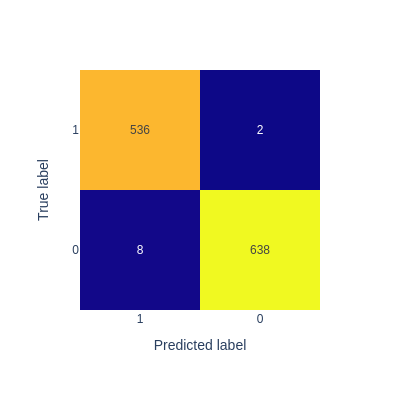
\includegraphics[scale=0.4]{/home/jacopo/PycharmProjects/muffin-stat-project/report/imgs/vgg16_confusion}
    \centering

    \begin{tabular}{ c | c | c | c| c}
        \hline
        reference  & $precision$ & $recall$ & $f1$   & $support$ \\
        \hline\hline
        muffin     & 0.9963      & 0.9853   & 0.9908 & 544       \\
        \hline
        chihuahua  & 0.9876      & 0.9969   & 0.9922 & 640       \\
        \hline
        $accuracy$ & -           & -        & 0.9916 & 1184      \\
        \hline
    \end{tabular}

    \caption{
        Metrics of the VGG-16 transfer learned model
    }\label{fig:figure6}
\end{figure}


It's hard to understand why the CNN models are underfitting, are the models too simple to capture the complexity
of the features?
If that were the case a good way to increase the performance could be adding more layer or simply more parameters.
Could the image augmentation technique be generating too noisy images?
Adding other samples to the dataset is another path worth considering as the dataset is not huge but so far, as expected, the more complex
and better trained pre-tuned models perform better under every aspect.

% confusion matrix V model finale (5)
% prec recall
% ROC?